\documentclass[8pt,a4paper,compress,handout]{beamer}

\usepackage{/home/siyer/lib/slides}

\title{Creating Data Types}
\date{}

\begin{document}
\begin{frame}
\vfill
\titlepage
\end{frame}

\begin{frame}
\frametitle{Outline}
\tableofcontents
\end{frame}

\section{Basic Elements of a Data Type}
\begin{frame}[fragile]
We implement a data type as a \emph{class} --- the keyword \lstinline{class}, followed by the class name, followed by a colon, and then a list of method definitions

\bigskip

A class typically defines a constructor, instance variables (aka attributes of the class), and methods

\bigskip

A constructor creates an object of the specified type and returns a reference to that object

\bigskip

When a client calls a constructor, Python calls the \lstinline{__init__()} method of the data type to define and initialize the instance variables, and returns a reference to the new object

\bigskip

A \emph{method} definition consists of its signature --- the \lstinline{def} keyword followed by its name, a list of parameter variables, and a colon --- and its body

\bigskip

By convention, the first parameter of a method is named \emph{self}

\bigskip

When a client calls a method, the \emph{self} parameter variable references the object to be manipulated, ie, the object that was used to invoke the method; in the case of \lstinline{__init__()}, it is a reference to the newly created object
\end{frame}

\begin{frame}[fragile]
\emph{Instance variables} implement the values of a data type 

\bigskip

An instance variable belongs to a particular instance of a class, ie, to a particular object 

\bigskip

By convention, instance variable names begin with an underscore

\bigskip

A method typically uses three kinds of variables
\begin{itemize}
\item The \lstinline{self} object's instance variables

\item The method's parameter variables

\item Local variables
\end{itemize}

\bigskip

The key difference between functions and methods is that a method is associated with a specified object, with direct access to its instance variables

\bigskip

To support the operation \lstinline{str(o)}, where \lstinline{o} is an object of data type \lstinline{T}, we must implement the method \lstinline{__str()__} in \lstinline{T}

\bigskip

A client should access a data type only through the methods in its API
\end{frame}

\section{Examples of Data Types}

\begin{frame}[fragile]
A data type \lstinline{Charge} for charged particles
\begin{center}
\begin{tabular}{cc}
method & description \\ \hline
\lstinline$Charge(x0, y0, q0)$ & a new charge $c$ centered at $(x_0, y_0)$ with charge value $q_0$ \\
\lstinline$c.potentialAt(x, y)$ & electric potential of charge $c$ at point $(x, y)$ \\
\lstinline$str(c)$ & string representation of charge $c$
\end{tabular} 
\end{center}
\end{frame}

\begin{frame}[fragile]
\begin{framed}
\tiny charge.py: Defines a data type \lstinline{Charge}. 
\end{framed}

\begin{lstlisting}[language=Python]
import math
import stdio
import sys

class Charge:
    def __init__(self, x0, y0, q0):
        self._rx = x0
        self._ry = y0
        self._q = q0

    def potentialAt(self, x, y):
        COULOMB = 8.99e09
        dx = x - self._rx
        dy = y - self._ry
        r = math.sqrt(dx * dx + dy * dy)
        if r == 0.0:
            return float('inf')
        return COULOMB * self._q / r

    def __str__(self):
        result = str(self._q) + ' at ('
        result += str(self._rx) + ', ' + str(self._ry) + ')'
        return result
\end{lstlisting}
\end{frame}

\begin{frame}[fragile]
\begin{lstlisting}[language=Python]
def main():
    x = float(sys.argv[1])
    y = float(sys.argv[2])
    c = Charge(.51, .63, 21.3)
    stdio.writeln(c)
    stdio.writeln(c.potentialAt(x, y))

if __name__ == '__main__':
    main()
\end{lstlisting}

\begin{lstlisting}[language={}]
$ python charge.py .5 .5
21.3 at (0.51, 0.63)
1.46863824819e+12
\end{lstlisting}
\end{frame}

\begin{frame}[fragile]
A data type \lstinline{Stopwatch} representing a stopwatch
\begin{center}
\begin{tabular}{cc}
method & description \\ \hline
\lstinline$Stopwatch()$ & a new stopwatch $w$ \\
\lstinline$w.elapsedTime()$ & elapsed time since $w$ was created, in seconds
\end{tabular} 
\end{center}
\end{frame}

\begin{frame}[fragile]
\begin{framed}
\tiny stopwatch.py: Defines a data type \lstinline{Stopwatch}. 
\end{framed}

\begin{lstlisting}[language=Python]
import stdio
import sys
import time

class Stopwatch:
    def __init__(self):
        self._creationTime = time.clock()
    
    def elapsedTime(self):
        return time.clock() - self._creationTime

def main():
    n = int(sys.argv[1])
    total1 = 0.0
    watch1 = Stopwatch()
    for i in range(1, n + 1):
        total1 += i ** 2
    time1 = watch1.elapsedTime()    
    total2 = 0.0
    watch2 = Stopwatch()
    for i in range(1, n + 1):
        total2 += i * i
    time2 = watch2.elapsedTime()    
    stdio.writef('%f\n%f\n', total1 / total2, time1 / time2)

if __name__ == '__main__':
    main()
\end{lstlisting}

\begin{lstlisting}[language={}]
$ python stopwatch.py 1000000
1.000000
1.280855
\end{lstlisting}
\end{frame}

\begin{frame}[fragile]
A data type \lstinline{Histogram} for graphically representing distributions of data
\begin{center}
\begin{tabular}{cc}
method & description \\ \hline
\lstinline$Histogram(n)$ & a new histogram $h$ from the integer values in $0, 1, \dots, n-1$ \\
\lstinline$h.addDataPoint(i)$ & add an occurrence of integer $i$ to the histogram $h$ \\
\lstinline$h.draw()$ & draw $h$ to standard draw
\end{tabular} 
\end{center}
\end{frame}

\begin{frame}[fragile]
\begin{framed}
\tiny histogram.py: Defines a data type \lstinline{Histogram}.
\end{framed}

\begin{lstlisting}[language=Python]
import stdarray
import stddraw
import stdrandom
import stdstats
import sys

class Histogram:
    def __init__(self, n):
        self._freqCounts = stdarray.create1D(n, 0)

    def addDataPoint(self, i):
        self._freqCounts[i] += 1

    def draw(self):
        stddraw.setYscale(0, max(self._freqCounts))
        stdstats.plotBars(self._freqCounts)

def main():
    n = int(sys.argv[1]) 
    p = float(sys.argv[2])
    trialCount = int(sys.argv[3]) 
    histogram = Histogram(n + 1)
    for trial in range(trialCount):
        heads = stdrandom.binomial(n, p)
        histogram.addDataPoint(heads)
    stddraw.setCanvasSize(500, 200)
    histogram.draw()
    stddraw.show()

if __name__ == '__main__':
    main()
\end{lstlisting}
\end{frame}

\begin{frame}[fragile]
\begin{minipage}{200pt}
\begin{lstlisting}[language={}]
$ python histogram.py 50 .5 1000000
\end{lstlisting}
\end{minipage}%
\hfill
\begin{minipage}{100pt}
\begin{center}
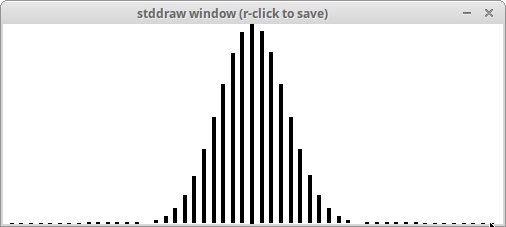
\includegraphics[scale=0.2]{figures/histogram1.png}

\smallskip

\tiny Binomial distribution ($n=50$, $p=0.5$)
\end{center}
\end{minipage}%

\bigskip

\begin{minipage}{200pt}
\begin{lstlisting}[language={}]
$ python histogram.py 50 .2 1000000
\end{lstlisting}
\end{minipage}%
\hfill
\begin{minipage}{100pt}
\begin{center}
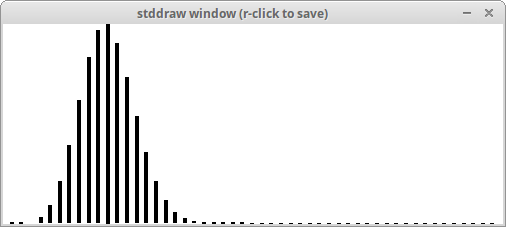
\includegraphics[scale=0.2]{figures/histogram2.png}

\smallskip

\tiny Binomial distribution ($n=50$, $p=0.2$)
\end{center}
\end{minipage}%

\bigskip

\begin{minipage}{200pt}
\begin{lstlisting}[language={}]
$ python histogram.py 50 .8 1000000
\end{lstlisting}
\end{minipage}%
\hfill
\begin{minipage}{100pt}
\begin{center}
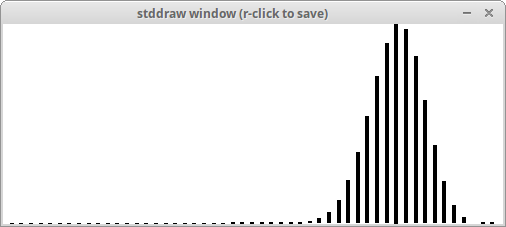
\includegraphics[scale=0.2]{figures/histogram3.png}

\smallskip

\tiny Binomial distribution ($n=50$, $p=0.8$)
\end{center}
\end{minipage}%
\end{frame}

\begin{frame}[fragile]
A data type \lstinline{Turtle} for producing turtle graphics
\begin{center}
\begin{tabular}{cc}
method & description \\ \hline
\lstinline$Turtle(x0, y0, a0)$ & a new turtle $t$ at $(x_0, y_0)$ facing $a_0$ degrees from the $x$-axis \\
\lstinline$t.turnLeft(delta)$ & instruct $t$ to turn left (conterclockwise) by $delta$ degrees \\
\lstinline$t.goForward(step)$ & instruct $t$ to move forward distance $step$, drawing a line
\end{tabular} 
\end{center}
\end{frame}

\begin{frame}[fragile]
\begin{framed}
\tiny turtle.py: Defines a data type \lstinline{Turtle}.
\end{framed}

\begin{lstlisting}[language=Python]
import math
import stddraw
import sys

class Turtle:
    def __init__(self, x, y, angle):
        self._x = x  
        self._y = y 
        self._angle = angle  
        
    def turnLeft(self, delta):
        self._angle += delta

    def goForward(self, step):
        oldx = self._x
        oldy = self._y
        self._x += step * math.cos(math.radians(self._angle))
        self._y += step * math.sin(math.radians(self._angle))
        stddraw.line(oldx, oldy, self._x, self._y)

def main():
    n = int(sys.argv[1])
    turtle = Turtle(.5, .0, 180.0 / n)
    stepSize = math.sin(math.radians(180.0 / n))
    for i in range(n):
        turtle.goForward(stepSize)
        turtle.turnLeft(360.0 / n)
    stddraw.show()

if __name__ == '__main__':
    main()
\end{lstlisting}
\end{frame}

\begin{frame}[fragile]
\begin{minipage}{200pt}
\begin{lstlisting}[language={}]
$ python turtle.py 3
\end{lstlisting}
\end{minipage}%
\hfill
\begin{minipage}{100pt}
\begin{center}
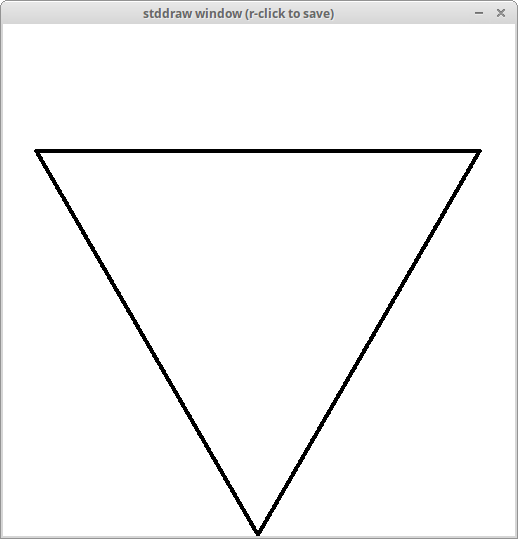
\includegraphics[scale=0.12]{figures/turtle1.png}

\smallskip

\tiny 3-sided polygon
\end{center}
\end{minipage}%

\bigskip

\begin{minipage}{200pt}
\begin{lstlisting}[language={}]
$ python turtle.py 7
\end{lstlisting}
\end{minipage}%
\hfill
\begin{minipage}{100pt}
\begin{center}
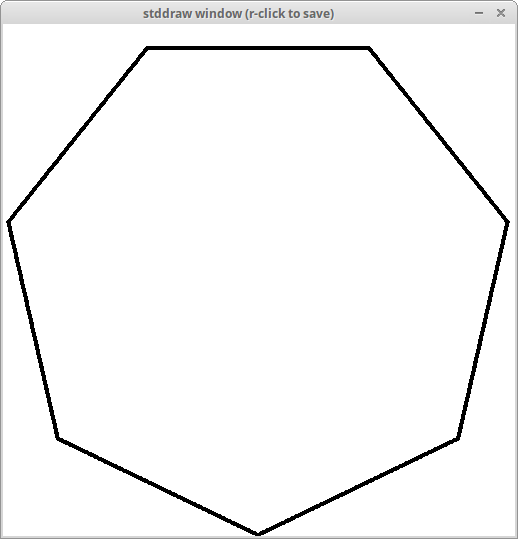
\includegraphics[scale=0.12]{figures/turtle2.png}

\smallskip

\tiny 7-sided polygon
\end{center}
\end{minipage}%

\bigskip

\begin{minipage}{200pt}
\begin{lstlisting}[language={}]
$ python turtle.py 30
\end{lstlisting}
\end{minipage}%
\hfill
\begin{minipage}{100pt}
\begin{center}
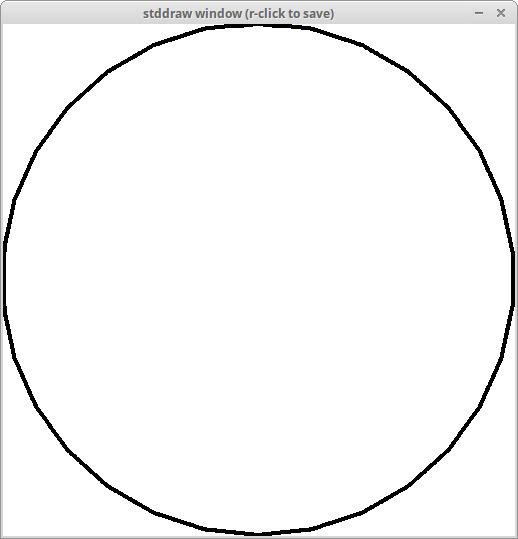
\includegraphics[scale=0.12]{figures/turtle3.png}

\smallskip

\tiny 30-sided polygon
\end{center}
\end{minipage}%
\end{frame}

\begin{frame}[fragile]
\begin{framed}
\tiny koch.py: Accepts integer $n$ as a command-line argument and plots a Koch curve of order $n$.
\end{framed}

\begin{lstlisting}[language=Python]
import stddraw
import sys
from turtle import Turtle

def koch(n, stepSize, myTurtle):
    if n == 0:
        myTurtle.goForward(stepSize)
        return  
    koch(n - 1, stepSize, myTurtle)
    myTurtle.turnLeft(60.0)
    koch(n - 1, stepSize, myTurtle)
    myTurtle.turnLeft(-120.0)
    koch(n - 1, stepSize, myTurtle)
    myTurtle.turnLeft(60.0)
    koch(n - 1, stepSize, myTurtle)
 
def main():
    n = int(sys.argv[1])
    stddraw.setCanvasSize(512, 256)
    stddraw.setYscale(-.1, 0.4)
    stddraw.setPenRadius(0.0)
    stepSize = 1.0 / (3.0 ** n)
    myTurtle = Turtle(0.0, 0.0, 0.0)
    koch(n, stepSize, myTurtle)
    stddraw.show()

if __name__ == '__main__':
    main()
\end{lstlisting}
\end{frame}

\begin{frame}[fragile]
\begin{minipage}{200pt}
\begin{lstlisting}[language={}]
$ python koch.py 0
\end{lstlisting}
\end{minipage}%
\hfill
\begin{minipage}{100pt}
\begin{center}
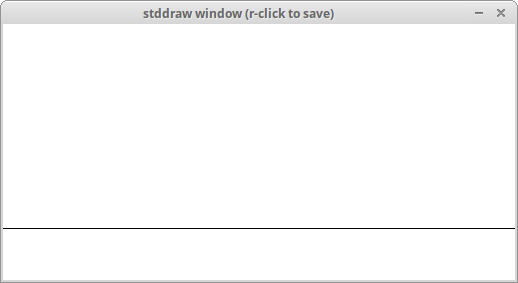
\includegraphics[scale=0.12]{figures/koch1.png}

\smallskip

\tiny Koch curve of order 0
\end{center}
\end{minipage}%

\bigskip

\begin{minipage}{200pt}
\begin{lstlisting}[language={}]
$ python koch.py 1
\end{lstlisting}
\end{minipage}%
\hfill
\begin{minipage}{100pt}
\begin{center}
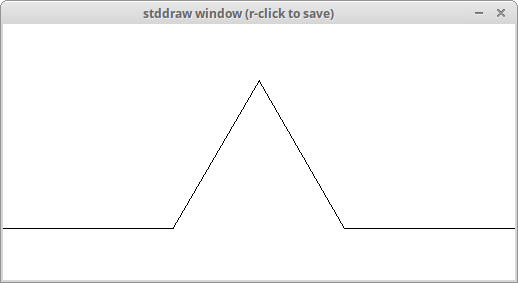
\includegraphics[scale=0.12]{figures/koch2.png}

\smallskip

\tiny Koch curve of order 1
\end{center}
\end{minipage}%

\bigskip

\begin{minipage}{200pt}
\begin{lstlisting}[language={}]
$ python koch.py 2
\end{lstlisting}
\end{minipage}%
\hfill
\begin{minipage}{100pt}
\begin{center}
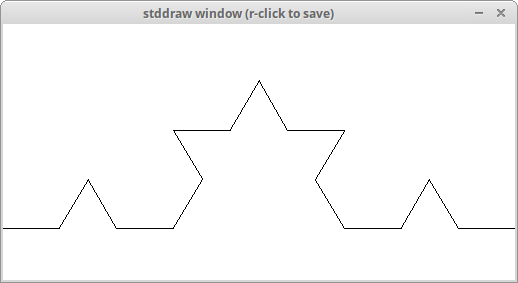
\includegraphics[scale=0.12]{figures/koch3.png}

\smallskip

\tiny Koch curve of order 2
\end{center}
\end{minipage}%

\bigskip

\begin{minipage}{200pt}
\begin{lstlisting}[language={}]
$ python koch.py 3
\end{lstlisting}
\end{minipage}%
\hfill
\begin{minipage}{100pt}
\begin{center}
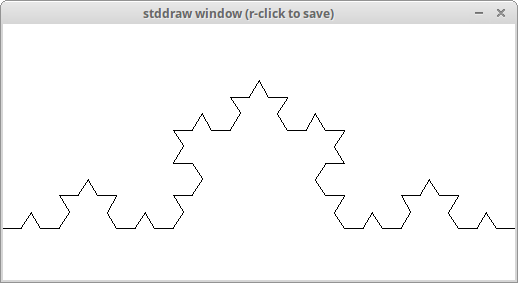
\includegraphics[scale=0.12]{figures/koch4.png}

\smallskip

\tiny Koch curve of order 3
\end{center}
\end{minipage}%

\bigskip

\begin{minipage}{200pt}
\begin{lstlisting}[language={}]
$ python koch.py 4
\end{lstlisting}
\end{minipage}%
\hfill
\begin{minipage}{100pt}
\begin{center}
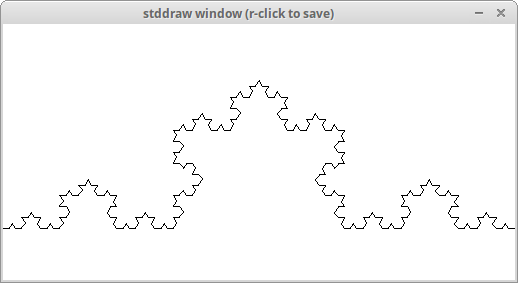
\includegraphics[scale=0.12]{figures/koch5.png}

\smallskip

\tiny Koch curve of order 4
\end{center}
\end{minipage}
\end{frame}

\begin{frame}[fragile]
\begin{framed}
\tiny spiral.py: Accepts command-line arguments $n$ (an integer specifying a number  of sides), $wraps$ (an integer specifying a wrap count), and $decay$ (a float specifying a decay factor), and draws a spiral with those characteristics.
\end{framed}

\begin{lstlisting}[language=Python]
import math
import stddraw
import sys
from turtle import Turtle

def main():
    n = int(sys.argv[1])
    wraps = int(sys.argv[2])
    decay = float(sys.argv[3])
    angle = 360.0 / n
    step = math.sin(math.radians(angle/2.0))
    turtle = Turtle(0.5, 0, angle/2.0)
    stddraw.setPenRadius(0.0)
    for i in range(wraps * n):
        step /= decay
        turtle.goForward(step)
        turtle.turnLeft(angle)
    stddraw.show()
    
if __name__ == '__main__':
    main()
\end{lstlisting}
\end{frame}

\begin{frame}[fragile]
\begin{minipage}{200pt}
\begin{lstlisting}[language={}]
$ python spiral.py 3 10 1.2
\end{lstlisting}
\end{minipage}%
\hfill
\begin{minipage}{100pt}
\begin{center}
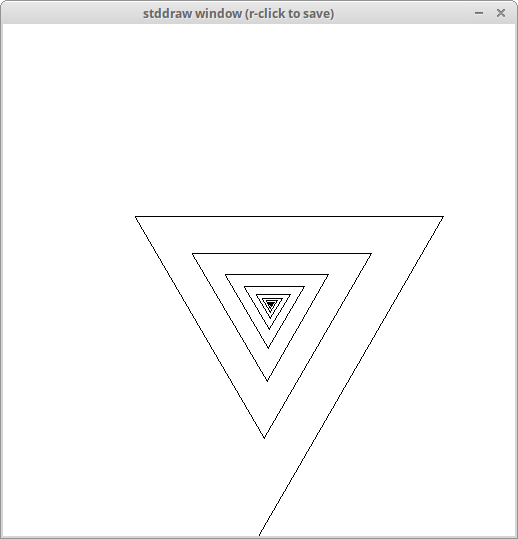
\includegraphics[scale=0.2]{figures/spiral1.png}

\smallskip

\tiny 3-sided outward spiral
\end{center}
\end{minipage}%

\bigskip

\begin{minipage}{200pt}
\begin{lstlisting}[language={}]
$ python spiral.py 1440 10 1.0004
\end{lstlisting}
\end{minipage}%
\hfill
\begin{minipage}{100pt}
\begin{center}
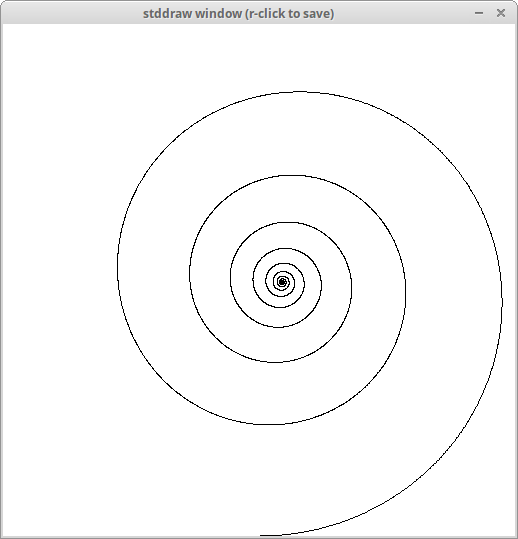
\includegraphics[scale=0.2]{figures/spiral2.png}

\smallskip

\tiny 1440-sided outward spiral
\end{center}
\end{minipage}
\end{frame}

\begin{frame}[fragile]
\begin{framed}
\tiny drunk.py: Accepts as command-line arguments an integer $stepCount$ specifying the number of iterations, and a float $stepSize$ specifying a step size, creates a \lstinline{Turtle} object, and has it make $stepCount$ random steps of size $stepSize$.
\end{framed}

\begin{lstlisting}[language=Python]
import stddraw
import stdrandom
import sys
from turtle import Turtle

def main():
    stepCount = int(sys.argv[1])
    stepSize = float(sys.argv[2])
    stddraw.setPenRadius(0.0)
    myTurtle = Turtle(0.5, 0.5, 0.0)
    for i in range(stepCount):
        myTurtle.turnLeft(360.0 * stdrandom.uniformFloat(0.0, 360.0))
        myTurtle.goForward(stepSize)
        stddraw.show(0.0)
    stddraw.show()

if __name__ == '__main__':
    main()
\end{lstlisting}
\end{frame}

\begin{frame}[fragile]
\begin{minipage}{200pt}
\begin{lstlisting}[language={}]
$ python drunk.py 10000 .01
\end{lstlisting}
\end{minipage}%
\hfill
\begin{minipage}{100pt}
\begin{center}
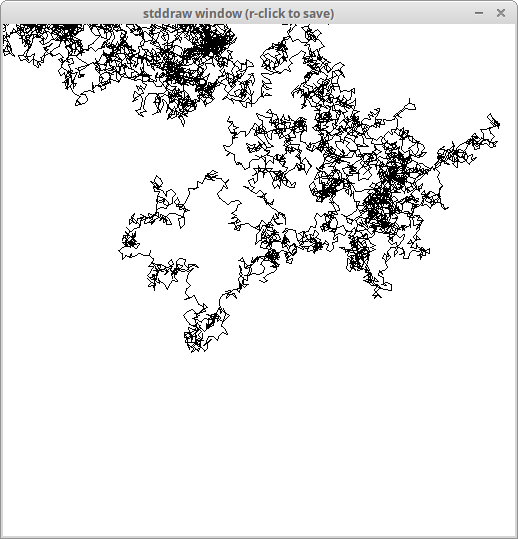
\includegraphics[scale=0.2]{figures/drunk.png}

\smallskip

\tiny One drunk turtle
\end{center}
\end{minipage}
\end{frame}

\begin{frame}[fragile]
\begin{framed}
\tiny drunks.py: Accepts as command-line arguments an integer $turtleCount$, an integer $stepCount$, and a float $stepSize$, creates $turtleCount$ \lstinline{Turtle} objects, and has them make $stepCount$ random steps of size $stepSize$.
\end{framed}

\begin{lstlisting}[language=Python]
import stdarray
import stddraw
import stdrandom
import sys
from turtle import Turtle

def main():
    turtleCount = int(sys.argv[1])
    stepCount = int(sys.argv[2])
    stepSize = float(sys.argv[3])
    stddraw.setPenRadius(0.0)
    turtles = stdarray.create1D(turtleCount)
    for i in range(turtleCount):
        x = stdrandom.uniformFloat(0.0, 1.0)
        y = stdrandom.uniformFloat(0.0, 1.0)
        turtles[i] = Turtle(x, y, 0.0)
    for j in range(stepCount):
        for i in range(turtleCount):
            turtles[i].turnLeft(stdrandom.uniformFloat(0.0, 360.0))
            turtles[i].goForward(stepSize)
            stddraw.show(0.0)
    stddraw.show()
    
if __name__ == '__main__':
    main()
\end{lstlisting}
\end{frame}

\begin{frame}[fragile]
\begin{minipage}{200pt}
\begin{lstlisting}[language={}]
$ python drunk.py 20 5000 .005
\end{lstlisting}
\end{minipage}%
\hfill
\begin{minipage}{100pt}
\begin{center}
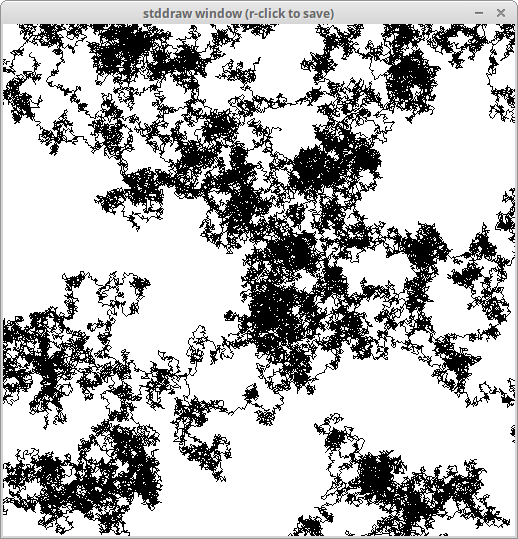
\includegraphics[scale=0.2]{figures/drunks.png}

\smallskip

\tiny 20 drunk turtles
\end{center}
\end{minipage}
\end{frame}

\begin{frame}[fragile]
A complex number is a number of the form $x+yi$, where $x$ (the real part) and $y$ (the imaginary part) are real numbers and $i=\sqrt{-1}$

\bigskip

Complex arithmetic
\begin{itemize}
\item Conjugate: $(x+yi)^\star=x-yi$

\item Addition: $(x+yi)+(v+wi) = (x+v) + (y+w)i$

\item Multiplication: $(x+yi)\times(v+wi) = (xv-yw) + (yv+xw)i$

\item Magnitude: $|x+yi|=\sqrt{x^2+y^2}$
\end{itemize}

\bigskip

A data type \lstinline{Complex} for representing complex numbers
\begin{center}
\begin{tabular}{cc}
method & description \\ \hline
\lstinline$Complex(x, y)$ & a new complex object $c$ with value $x + yi$ \\
\lstinline$c.re()$ & real part of $c$ \\
\lstinline$c.im()$ & imaginary part of $c$ \\
\lstinline$c.conjugate()$ & conjugate of $c$ \\
\lstinline$c + d$ & sum of $c$ and $d$ \\
\lstinline$c * d$ & product of $c$ and $d$ \\
\lstinline$abs(c)$ & magnitute of $c$ \\
\lstinline$str(c)$ & \lstinline$x + yi$ (string representation of $c$)
\end{tabular} 
\end{center}
\end{frame}

\begin{frame}[fragile]
\begin{framed}
\tiny complex.py: Defines a data type \lstinline{Complex}.
\end{framed}

\begin{lstlisting}[language=Python]
import math
import stdio

class Complex:
    def __init__(self, re = 0.0, im = 0.0):
        self._re = re
        self._im = im

    def re(self):
        return self._re

    def im(self):
        return self._im

    def conjugate(self):
        return Complex(self._re, -self._im)

    def __add__(self, other):
        re = self._re + other._re
        im = self._im + other._im
        return Complex(re, im)

    def __mul__(self, other):
        re = self._re * other._re - self._im * other._im
        im = self._re * other._im + self._im * other._re
        return Complex(re, im)
\end{lstlisting}
\end{frame}

\begin{frame}[fragile]
\begin{lstlisting}[language=Python]
    def __abs__(self):
        return math.sqrt(self._re * self._re + self._im * self._im)

    def __str__(self):
        return str(self._re) + ' + ' + str(self._im) + 'i'

def main():
    z0 = Complex(1.0, 1.0)
    z = z0
    z = z * z + z0
    z = z * z + z0
    stdio.writeln(z)

if __name__ == '__main__':
    main()
\end{lstlisting}

\begin{lstlisting}[language={}]
$ python complex.py 
-7.0 + 7.0i
\end{lstlisting}
\end{frame}

\begin{frame}[fragile]
\begin{framed}
\tiny mandelbrot.py: Accepts float command-line arguments $xc$, $yc$, and $size$ that specify the center and size of a square region of interest, and makes a digital image showing the result of sampling the Mandelbrot set in that region. The algorithm is as follows:
\begin{itemize}
\item Consider $z_0, z_1, \dots, z_t$, where $z_{t+1}=z_t^2+z_0$
\item If the sequence $|z_t|$ diverges to infinity, then $z_0$ is not in the Mandelbrot set; if the sequence is bounded, then $z_0$ is in the set
\end{itemize}
\end{framed}

\begin{lstlisting}[language=Python]
import stddraw
import sys
from color import Color
from complex import Complex
from picture import Picture

def mandel(z0, limit):
    z = z0
    for t in range(limit):
        if abs(z) > 2.0:
            return t
        z = z * z + z0
    return limit

def main():
    MAX = 255
    n = int(sys.argv[1])
    xc = float(sys.argv[2])
    yc = float(sys.argv[3])
    size = float(sys.argv[4])
    pic = Picture(n, n)
\end{lstlisting}
\end{frame}

\begin{frame}[fragile]
\begin{lstlisting}[language=Python]
    for col in range(n):
        for row in range(n):
            x0 = xc - (size / 2) + (size * col / n)
            y0 = yc - (size / 2) + (size * row / n)
            z0 = Complex(x0, y0)
            gray = MAX - mandel(z0, MAX)
            color = Color(gray, gray, gray)
            pic.set(col, n - 1 - row, color)
    stddraw.setCanvasSize(n, n)
    stddraw.picture(pic)
    stddraw.show()

if __name__ == '__main__':
    main()
\end{lstlisting}
\end{frame}

\begin{frame}[fragile]
\begin{minipage}{200pt}
\begin{lstlisting}[language={}]
$ python mandelbrot.py 512 -.5 0 2
\end{lstlisting}
\end{minipage}%
\hfill
\begin{minipage}{100pt}
\begin{center}
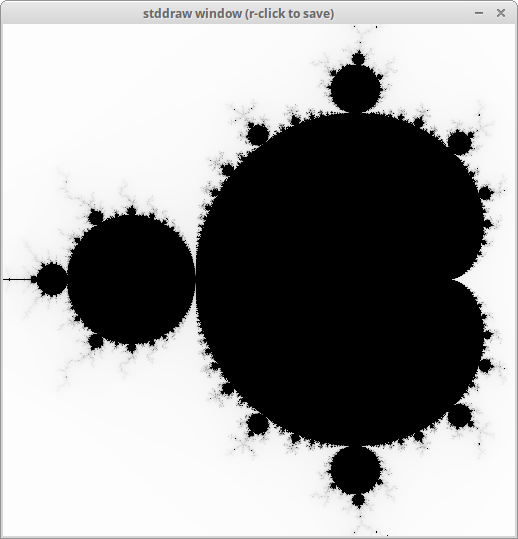
\includegraphics[scale=0.2]{figures/mandelbrot1.png}

\smallskip

\tiny Mandelbrot set
\end{center}
\end{minipage}%

\bigskip

\begin{minipage}{200pt}
\begin{lstlisting}[language={}]
$ python mandelbrot.py 512 .1015 -.633 .01
\end{lstlisting}
\end{minipage}%
\hfill
\begin{minipage}{100pt}
\begin{center}
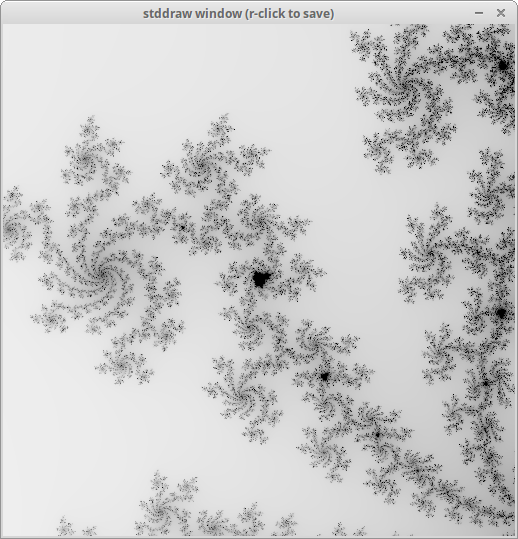
\includegraphics[scale=0.2]{figures/mandelbrot2.png}

\smallskip

\tiny A portion of the Mandelbrot set
\end{center}
\end{minipage}%
\end{frame}

\begin{frame}[fragile]
A data type \lstinline{StockAccount} for maitaining customer accounts containing shares of various stocks
\begin{center}
\begin{tabular}{cc}
method & description \\ \hline
\lstinline$StockAccount(filename)$ & a new account $a$, created from data from file $filename$ \\
\lstinline$a.valueOf()$ & total value of account $a$ \\
\lstinline$a.write(filename)$ & write account $a$ to $filename$ \\
\lstinline$a.writeReport()$ & write to standard output a detailed report for account $a$
\end{tabular} 
\end{center}
\end{frame}

\begin{frame}[fragile]
\begin{framed}
\tiny stockaccount.py: Accepts as a command-line argument the name of a file, reads from the file to create a \lstinline{StockAccount} object, and writes a report to standard output.
\end{framed}

\begin{lstlisting}[language=Python]
import stdarray
import stdio
import stockquote
import sys
from instream import InStream
from outstream import OutStream

class StockAccount:
    def __init__(self, filename):
        inStream = InStream(filename)
        self._name = inStream.readLine()
        self._cash = inStream.readFloat()
        self._stockCount = inStream.readInt()
        self._stocks = stdarray.create1D(self._stockCount, 0)
        self._shares = stdarray.create1D(self._stockCount, 0)
        for i in range(self._stockCount):
            self._shares[i] = inStream.readInt()
            self._stocks[i] = inStream.readString()

    def valueOf(self):
        total = self._cash
        for i in range(self._stockCount):
            price = stockquote.priceOf(self._stocks[i])
            amount = self._shares[i]
            total += amount * price
        return total
\end{lstlisting}
\end{frame}

\begin{frame}[fragile]
\begin{lstlisting}[language=Python]
    def write(self, filename):
        outStream = OutStream(filename)
        outStream.writeln(self._name)
        outStream.writeln(self._cash)
        outStream.writeln(self._stockCount)
        for i in range(self._stockCount):
            outStream.writef('%3d', self._shares[i])
            outStream.write(' ')
            outStream.writeln(self._stocks[i])

    def writeReport(self):
        stdio.writeln(self._name)
        total = self._cash
        for i in range(self._stockCount):
            amount = self._shares[i]
            price = stockquote.priceOf(self._stocks[i])
            total += amount * price
            stdio.writef('%4d  %4s ', amount, self._stocks[i])
            stdio.writef('  %7.2f   %9.2f\n', price, amount * price)
        stdio.writef('%21s %10.2f\n', 'Cash:', self._cash)
        stdio.writef('%21s %10.2f\n', 'Total:', total)

def main():
    acct = StockAccount(sys.argv[1])
    acct.writeReport()

if __name__ == '__main__':
    main()
\end{lstlisting}
\end{frame}

\begin{frame}[fragile]
\begin{lstlisting}[language={}]
$ more turing.txt 
Turing, Alan
10.24
4
100 ADBE
 25 GOOG
 97 IBM
250 MSFT
$ python stockaccount.py turing.txt 
Turing, Alan
 100  ADBE     91.32     9132.00
  25  GOOG    740.34    18508.50
  97   IBM    135.21    13115.37
 250  MSFT     54.10    13525.00
                Cash:      10.24
               Total:   54291.11
\end{lstlisting}
\end{frame}
\end{document}
